
\begin{figure}
  \centering
  \hspace*{\fill}
  \subfigure[]{\label{subfig:1a}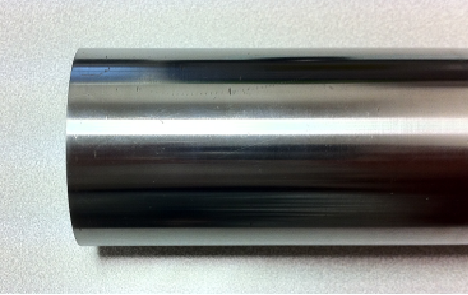
\includegraphics[width=0.15\linewidth]{./Figure/Figure1/A1.png}} \hfill
  \subfigure[]{\label{subfig:1b}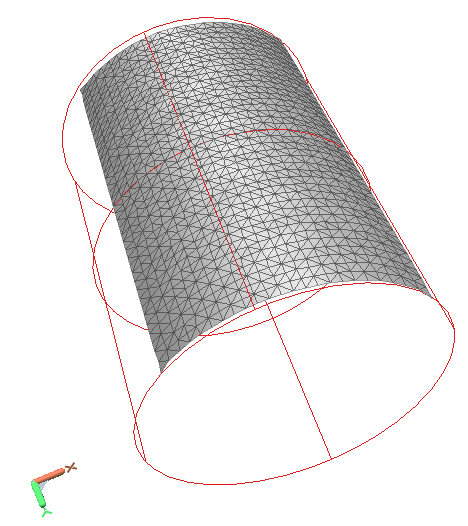
\includegraphics[width=0.15\linewidth]{./Figure/Figure1/A2.png}} \hfill
  \subfigure[]{\label{subfig:1c}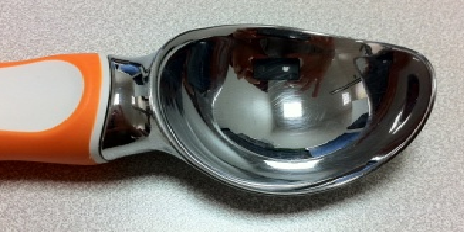
\includegraphics[width=0.15\linewidth]{./Figure/Figure1/B1.png}} \hfill
  \subfigure[]{\label{subfig:1d}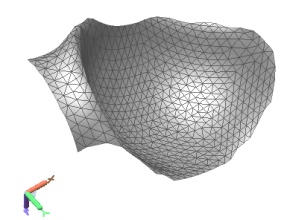
\includegraphics[width=0.15\linewidth]{./Figure/Figure1/B2.png}}
  \hspace*{\fill} \\ \hspace*{\fill}
  \subfigure[]{\label{subfig:1e}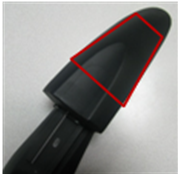
\includegraphics[width=0.15\linewidth]{./Figure/Figure1/C1.png}} \hfill
  \subfigure[]{\label{subfig:1f}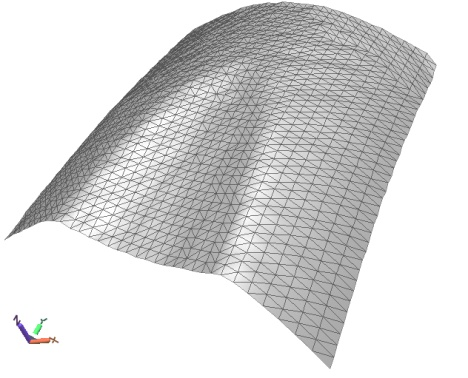
\includegraphics[width=0.15\linewidth]{./Figure/Figure1/C2.png}} \hfill
  \subfigure[]{\label{subfig:1g}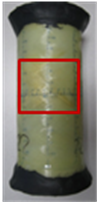
\includegraphics[width=0.1\linewidth]{./Figure/Figure1/D1.png}} \hfill
  \subfigure[]{\label{subfig:1h}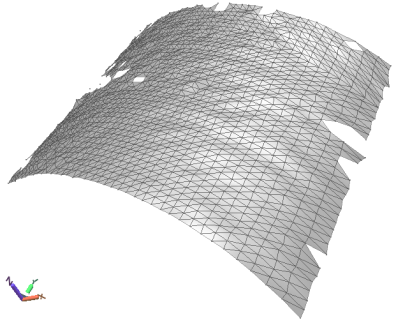
\includegraphics[width=0.15\linewidth]{./Figure/Figure1/D2.png}}
  \hspace*{\fill} \\ \hspace*{\fill}
  \subfigure[]{\label{subfig:1i}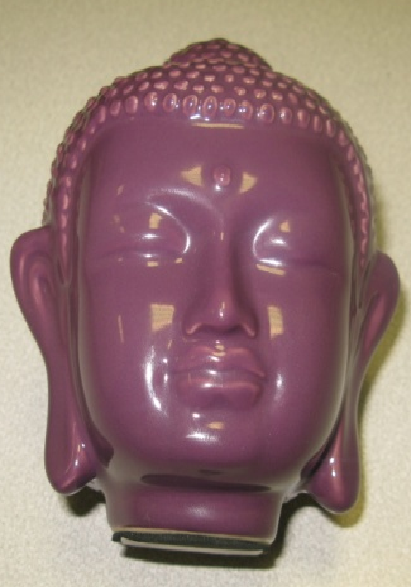
\includegraphics[width=0.15\linewidth]{./Figure/Figure1/E1.png}} \hfill
  \subfigure[]{\label{subfig:1j}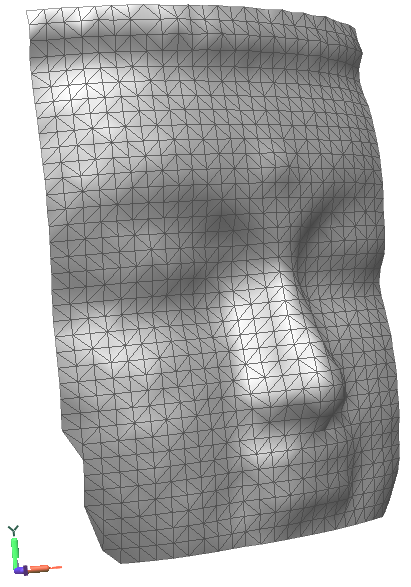
\includegraphics[width=0.15\linewidth]{./Figure/Figure1/E2.png}} \hfill
  \subfigure[]{\label{subfig:1k}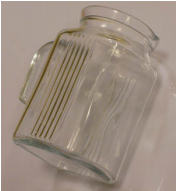
\includegraphics[width=0.15\linewidth]{./Figure/Figure1/F1.png}} \hfill
  \subfigure[]{\label{subfig:1l}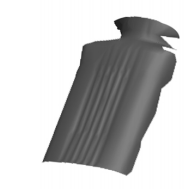
\includegraphics[width=0.15\linewidth]{./Figure/Figure1/F2.png}}
  \hspace*{\fill}
	  \caption{Examples of 3D digitization obtained by \acs*{sfh} approach: (a), (b), (c) and (d) metallic specular surfaces \cite{bajard2013numerisation} - (e) and (f) black plastic - (g) and (h) composite material - (i) and (j) ceramic - (k) and (l) glass transparent object \cite{meriaudeau20113d}.}
  \label{fig:1}
\end{figure}
